\section{Implementierungsdetails} \label{sec:implementation_misc}

In folgendem Kapitel wird die Implementierung der Anwendung näher beschrieben. Hierzu wird zunächst in Kapitel \ref{ssec:payload-generation} der Programmablauf näher betrachtet. Im Anschluss daran werden in \ref{ssec:components} die entwickelten Komponenten, Klassen sowie Designentscheidungen erläutert. Zuletzt wird in den Kapiteln \ref{ssec:initializing} und \ref{ssec:configuration} erläutert, wie die Initialisierungsphase und Konfiguration der Anwendung gesteuert werden können.

\subsection{Programmablauf}\label{ssec:payload-generation}
Im weiteren Verlauf der Arbeit wird davon ausgegangen, dass eine SUT-Konfiguration gegeben ist. Dies hat zur Folge, dass der Programmablauf von SmartGrazer dem Ablaufdiagramm aus Abbildung \ref{fig:SmartGrazerWorkflowPhases} entspricht. Das Ablaufdiagramm und dessen einzelne Phasen werden im Folgenden genauer betrachtet.

Die gezeigten Phasen finden nach der Initialisierung des Programms statt. Phase eins (Abbildung \ref{fig:SmartGrazer-workflow-phase1}) umfasst das Senden einer validen Anfrage und deren Analyse. Zusätzlich wird in dieser Phase ein Response-Objekt erstellt, mit dem im weiteren Verlauf des Testlaufs gearbeitet wird.

\begin{figure}[htbp] 
	\centering
	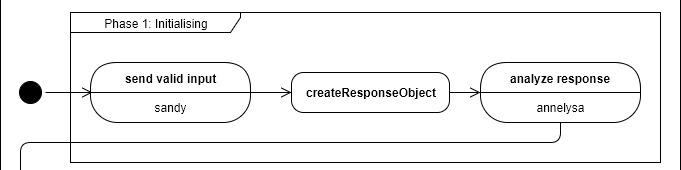
\includegraphics[width=.95\textwidth]{contents/images/SmartGrazerWorkflowPhase1}
	\caption{SmartGrazer: Programmablauf Phase 1}
	\label{fig:SmartGrazer-workflow-phase1}
\end{figure}

\FloatBarrier

In der zweiten Phase (Abbildung \ref{fig:SmartGrazer-workflow-phase2}) werden mehrerer Anfragen gesendet, um die ersten Anpassungen der Elemente vorzunehmen. Eine dieser Anfragen umfasst eine Liste von Sonderzeichen. Die in dieser Phase verwendeten Payloads werden statisch definiert und gelten in jedem Durchlauf von SmartGrazer. Der verwendete Generator ``Simpy'' konfiguriert die ersten Elemente für den eigentlichen Payload-Generator ``Smarty'' vor.

\begin{figure}[htbp] 
	\centering
	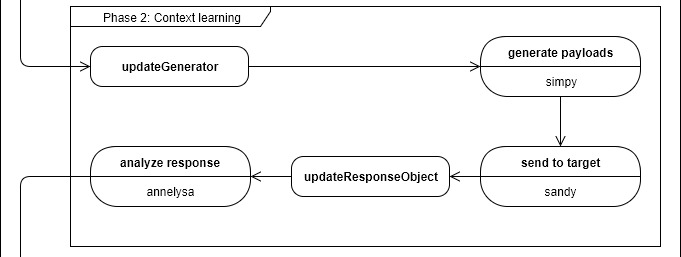
\includegraphics[width=.95\textwidth]{contents/images/SmartGrazerWorkflowPhase2}
	\caption{SmartGrazer: Programmablauf Phase 2}
	\label{fig:SmartGrazer-workflow-phase2}
\end{figure}

\FloatBarrier

In Phase drei (Abbildung \ref{fig:SmartGrazer-workflow-phase3}) beginnt die eigentliche Konstruktion eines reflektierenden bzw. ausführbaren Payloads.

\begin{figure}[htbp] 
	\centering
	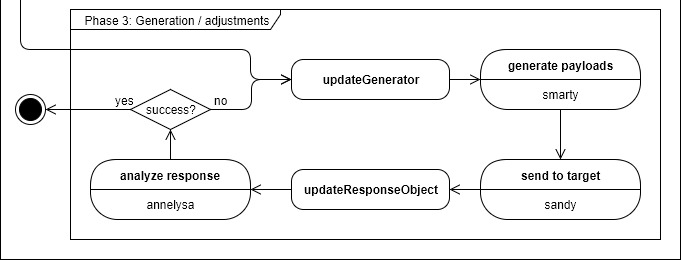
\includegraphics[width=.95\textwidth]{contents/images/SmartGrazerWorkflowPhase3}
	\caption{SmartGrazer: Programmablauf Phase 3}
	\label{fig:SmartGrazer-workflow-phase3}
\end{figure}

\FloatBarrier

\subsection{Komponentenübersicht und Klassendiagramm}\label{ssec:components}

In Abbildung \ref{fig:component-diagram} sind die wichtigsten Komponenten der Applikation und deren Verbindungen zueinander abgebildet. Durch das Aufteilen eines Testlaufs in viele kleine Teilaufgaben, entstanden im Laufe der Implementierung die gezeigten Hauptkomponenten. Wie später vorgestellt wird, teilen sich diese in mehrere Klassen auf. Als Hauptaufgaben eines Testlaufs wurden neben der Verarbeitung von Benutzereingaben, die Konfiguration, die Generierung, die Kommunikation mit dem SUT, die Analyse, Mutation und Anpassung von Payloads identifiziert.

Jede Komponente, die eine Teilaufgabe übernimmt, wurde mit einem Namen versehen, um eine Verständnisgrundlage zu schaffen. Grund hierfür ist, dass einige Komponenten identisch aufgebaut sind, jedoch verschiedene Funktionsweisen aufweisen.

Anhand des vereinfachten Klassendiagramms (Abbildung \ref{fig:simple-class-diagram})  ist erkennbar, wie die identifizierten Komponenten implementiert wurden. Die Färbung der Komponenten wird hierbei in der Abbildung \ref{fig:simple-class-diagram} übernommen, sodass die implementierten Klassen den entsprechenden Komponenten zugeordnet werden können.

\begin{figure}[htbp] 
	\centering
	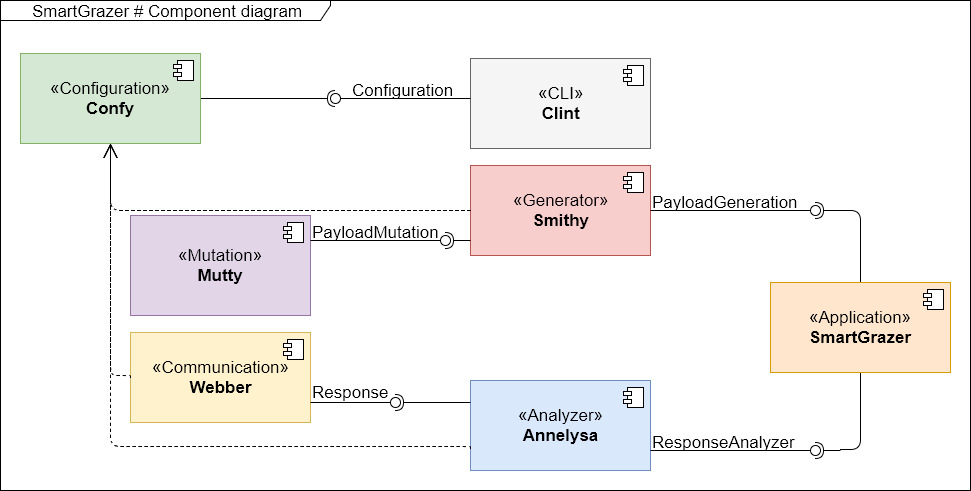
\includegraphics[width=\textwidth]{contents/images/SmartGrazerComponentDiagram}
	\caption{Smartgrazer: Komponentendiagramm}
	\label{fig:component-diagram}
\end{figure}

Die in Abbildung \ref{fig:component-diagram} aufgeführte Generierungs-Komponente ``Smithy'' ist während der Implementierung in mehrere Klassen aufgeteilt worden. Wichtigsten Bestandteile sind die Elemente und deren Lebenspunkte, beide definiert durch die Klassen ``Element'' bzw. ``Life''. Verschiedene Payload-Generatoren sind durch die Klassen ``PayloadGeneratorFactory'', ``GeneratorGeneral'' und ``PayloadGenerator'' realisiert.

\begin{figure}[htbp] 
	\centering
	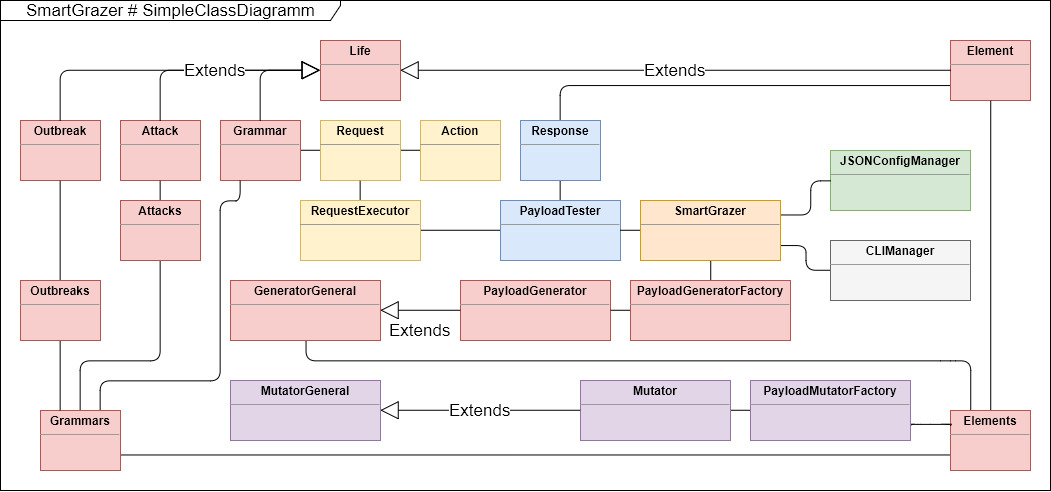
\includegraphics[width=\textwidth]{contents/images/SmartGrazerSimpleClassDiagram}
	\caption{SmartGrazer: Vereinfachtes Klassendiagramm}
	\label{fig:simple-class-diagram}
\end{figure}

Die Klasse ``PayloadGenerator'' wird von drei Generatoren (Dharma, Smarty und Simpy) implementiert, welche durch die Namensgebung in verschiedenen Python-Modulen liegen. Hierdurch kann während der Laufzeit die richtige Klasse von der Fabrik geladen und instanziiert werden.

Die generierten Payloads setzen sich durch ein Zusammenspiel der Klassen ``Outbreak'', ``Attack'' und ``Grammar'' zusammen. aKlassen der Mutations-Komponente sind durch die gleiche Vorgehensweise realisiert wie die Generator-Klassen.
\FloatBarrier
\paragraph{Instanziierung via Fabric-Pattern}

Durch die Verwendung von mehreren Generator- und Mutations-Klassen ist die eigentliche Instanziierung als Fabrik-Entwurfsmuster realisiert. Dieses Muster ist besonders geeignet für Objekte, die zur Laufzeit initialisiert werden müssen. Im Falle der ``PayloadGeneratorFactory'' (Komponente: Smithy) wird während der Ausführung zwischen den Generatoren ``Dharma'' und ``Smarty'' gewählt. Während der Programmausführung wird über die Fabrik-Klasse ``Smithy'' mit der geladenen Generator-Klasse kommuniziert. In Abbildung \ref{fig:SmartGrazer-Fabric-Pattern} ist exemplarisch das Muster für die Generator-Klassen abgebildet.

\begin{figure}[htbp] 
	\centering
	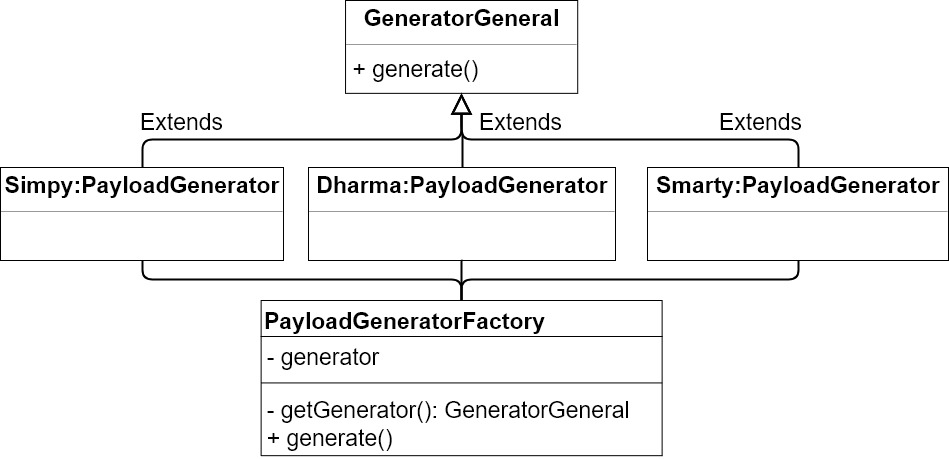
\includegraphics[width=.9\textwidth]{contents/images/SmartGrazerFabricPattern}
	\caption{SmartGrazer: Generator-Klassen als Fabrik-Entwurfsmuster}
	\label{fig:SmartGrazer-Fabric-Pattern}
\end{figure}

Die Verwendung dieses Entwurfsmusters ermöglicht  ein einfaches Hinzufügen und Verwenden von zusätzlichen Generator-Implementierungen.

\FloatBarrier

\subsection{Initiierung}\label{ssec:initializing}

Zu Beginn eines Testlaufs werden alle benötigten Element-Objekte geladen und mit einem Startwert für deren Leben initiiert. Aus Erfahrung sind einige Elemente öfter bzw. besser für \ac{XSS}-Angriffe geeignet und können seinen höheren Startwert zugewiesen bekommen als Elemente mit selteneren Verwendung. 

Da Elemente eine wichtige Rolle für die Generierung von Payloads haben, können diese in besonders hohem Maß konfiguriert werden. Zum aktuellen Stand der Implementierung können Elemente durch drei Konfigurationsdateien angepasst werden.

\paragraph{config/smarty/elements.json} Liste aller verfügbarer Elemente mit Verwendungszwecken. Als Verwendungszweck werden hier die Element-Schlüssel aus den Angriffsmustern bezeichnet. Dies ist notwendig, da manche Zeichen mehrere Aufgaben bzw. Bedeutungen in Payloads besitzen können. Im Beispiel \ref{lst:element-example-with-usage} wurden dem ``/''-Zeichen insgesamt drei Verwendungen (Leerraum, Schrägstrich und dem Wert eines ``SRC''-Elements) zugewiesen.

\begin{lstlisting}[caption={SmartGrazer: Auszug der Konfigurationsdatei ``elements.json''},label=lst:element-example-with-usage]
...
"47": [
  "SPACE",
  "SLASH",
  "SRC_VALUE"
], ...
\end{lstlisting}

\paragraph{config/smarty/elements.life.json} Liste aller Elemente mit den entsprechenden Lebenspunkten beim Start des Programmaufrufs. In Beispiel \ref{lst:element-life-example} ist ein Ausschnitt der Konfiguration dargestellt. Oft verwendete Elemente, wie z.B. das ``video''-Tag sind hier mit den maximalen Lebenspunkten ausgewiesen. Weniger häufig verwendete Elemente werden dementsprechend mit weniger Leben initialisiert.
	
\begin{lstlisting}[caption={SmartGrazer: Auszug der Konfigurationsdatei ``elements.life.json''},label=lst:element-life-example]
...
"var": 50,
"video": 100,
"wbr": 25,
"onclick": 25,
"ondblclick": 25,
...
\end{lstlisting}

	
\paragraph{config/smarty/elements.mutator.json} Liste aller Mutationsklassen und den dafür erlaubten Elementen. Beispiel \ref{lst:element-mutator-example} zeigt die Konfiguration der Mutator-Klasse ``Uppy'' und die freigeschalteten Elementen.

\begin{lstlisting}[caption={SmartGrazer: Auszug der Konfigurationsdatei ``elements.mutator.json''},label=lst:element-mutator-example]
...
"uppy": {
  "enabled": true,
  "elements": [
    "TAG_HMTL",
    "TAG_JS",
    "TAG_SCRIPT",
    "EVENT",
    "TEXT"
  ]
},
...
\end{lstlisting}

Der Zeitpunkt der Mutation findet unmittelbar nach der Ziehung des verwendeten Zeichens bzw. der verwendeten Zeichenkette statt. Der mutierte Wert des Elements wird hierbei in einer eigenen Variable gespeichert, welche bei der Ausgabe des Element-Wertes ausgegeben wird. Falls bei der Analyse der Webseitenantwort der mutierte Wert nicht reflektiert wurde, werden die Lebenspunkte des Elements verringert. 

\subsection{Konfiguration und Programmaufruf}\label{ssec:configuration}

Die Konfigurationsdateien werden im \gls{JSON}-Format gepflegt. Dies hat den Vorteil, dass auf die eingelesenen Daten, während der Laufzeit zugegriffen werden kann - vergleichbar zu Objekten. Zusätzlich kann jede Konfigurationsoption beim Aufruf von SmartGrazer über die Option --overwrite für den aktuellen Aufruf geändert werden.

Das \ac{CLI} ist mit der Python-Erweiterung ``argparse'' realisiert. In Abbildung \ref{fig:smartgrazer-cli-help} ist die Hilfe-Seite der Anwendung dargestellt. Der Flag-Parameter -g generiert Payloads und gibt diese danach aus. Über den Parameter -x wird SmartGrazer eine \ac{SUT}-Konfiguration übergeben, für die ein funktionierender Payload ermittelt werden soll. Die Optionen -g und -x sind gegenseitig ausschließend, d. h. nur eine der beiden Optionen kann bei einem Aufruf ausgewählt werden. 

\begin{figure}[htbp] 
	\centering
	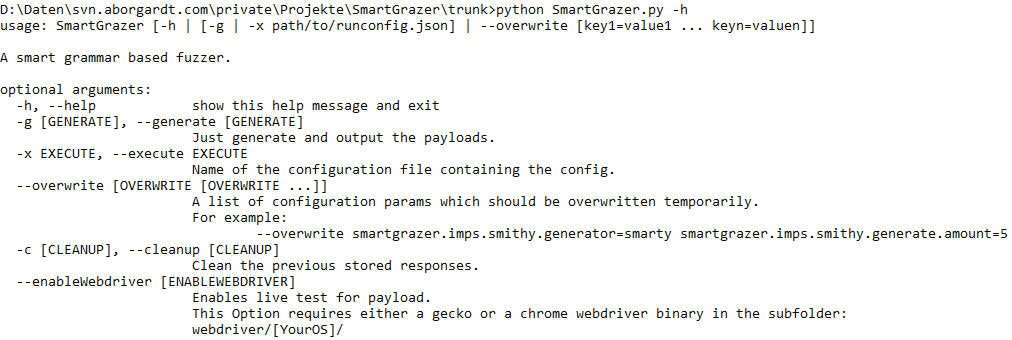
\includegraphics[width=\textwidth]{contents/images/SmartGrazerCLIHelp}
	\caption{SmartGrazer: Hilfe des Kommandozeilenprogramms}
	\label{fig:smartgrazer-cli-help}
\end{figure}

\FloatBarrier
Die Einstellungen für die Applikation und die enthaltenen Komponenten werden in der Datei ``config/config.json'' gepflegt.

Wird der Flag-Parameter ``-c'' angegeben, werden alle temporären Dateien vor dem Beginn der Generierung gelöscht. Durch Anhängen des ``--enableWebdriver''-Flags wird eine zusätzliche Testinstanz von SmartGrazer aktiviert. Diese führt dazu, dass SmartGrazer solange Payloads generiert, bis eine ``alert''-Box erzeugt werden konnte.

\subsubsection{Temporäres Überschreiben der Konfiguration}

Der ``--overwrite''-Parameter erwartet eine Schlüssel-Wert-Liste, welche mit einem Leerzeichen getrennt ist. Eine beispielhafte Anwendung dieses Parameters ist auf der Hilfe-Seite der Applikation aufgeführt.

\begin{figure}[htbp] 
	\centering
	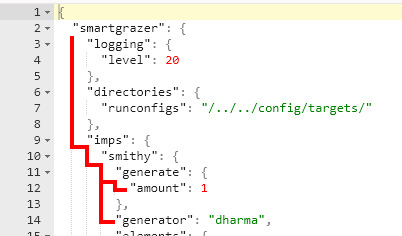
\includegraphics[width=0.65\textwidth]{contents/images/JSONConfigOverwritePath}
	\caption{SmartGrazer: Auszug der Konfigurationsdatei ``config/config.json''}
	\label{fig:config-json}
\end{figure}

\FloatBarrier
Die Notation der Schlüssel-Wert-Paare ist hierbei identisch mit dem Pfad in der dazugehörigen JSON-Konfigurationsdatei, wie in Abbildung \ref{fig:config-json} zu sehen ist. Für die gegebenen Beispiele (``smartgrazer.imps.smithy.generator=smarty'' und\\ ``smartgrazer.imps.smithy.generate.amount=5'') ist für den Parameter ``--overwrite'' in Abbildung \ref{fig:config-json} der Baumpfad mit roter Farbe markiert. Die Zuweisung neuer Werte erfolgt mit einem Gleich-Zeichen. Getrennt werden Schlüssel-Wert-Paare mit einem Leerzeichen. Im gezeigten Beispiel wird der Generator ``dharma'' durch ``smarty'' ersetzt und die Anzahl an generierten Payloads von ``1'' auf ``5'' erhöht.

Neben der beschriebenen ``config.json''-Datei kann eine Konfiguration für jede beliebige Webseite angelegt werden. Optionen dieser Konfigurationsdatei können ebenfalls durch den ``--overwrite''-Parameter überschrieben werden.
